\head{Ноябрь}{Листок 4. Теория чисел. Уровень 2.}

\begin{thm}
    Докажите, что число не может попасть в два разных класса (т.е. что число не может давать двух различных остатков при делении на одно и то же число).\footnote{Другими словами мы просим вас доказать корректность определения деления с остатком.}
\end{thm}
    
\begin{thm}
    Можно ли разрезать 6 прутьев длиной по 1 м каждый на 10 кусков длиной 27 см, 16 кусков длиной 15 см и 15 кусков длиной 6 см?
\end{thm}

\begin{thm}
    Докажите, что при любом натуральном $n$ число $n^3 + 3n^2 + 2n$ кратно 6.
\end{thm}

\begin{thm}
    Докажите, что при любом натуральном $n$ число $n(n + 1)^2(3n + 2)$ кратно 4.
\end{thm}

\begin{thm}
    Докажите, что для любого простого $p > 3$ число $p^2 - 1$ делится на 24.
\end{thm}

\begin{thm} $^n$ \label{4.2 thm1}
    Докажите, что при любом натуральном $n$ число $n^3 + 5n$ делится на 3. 
\end{thm}  

\begin{center}
Для решения следующих двух задач рекомендуется вспомнить задачи из предыдущего листка. 
\end{center}

\begin{thm} Докажите, что
    \par 
    а)~из 8 целых чисел всегда можно выбрать два таких, разность которых делится на 7. 
    \par 
    б)~из 5 чисел всегда можно выбрать два таких, у которых разность квадратов делится на 7.
\end{thm}

\begin{thm}
    Докажите, что среди чисел, написанных только единицами найдётся число,
    \\
    делящееся на 2012.
\end{thm}

\begin{thm}
    Докажите, что сумма квадратов двух последовательных целых чисел при делении на 4 даст остаток 1.
\end{thm}

\begin{thm}
    Докажите, что, если число $a^2 + b^2$ делится на 7, то числа $a$ и $b$ делятся на 7.
\end{thm}

\begin{thm} $^n$ \label{4.2 thm2} 
    Число $a$ - чётное, не кратное 4. Докажите, что число $a^2$ при делении на 32 даст остаток 4.
\end{thm}

\begin{thm}
    Число $a$ не делится ни на 2, ни на 3. Найдите остаток от деления числа $a^2$ на 6.
\end{thm}

\fbox{\begin{minipage}{0.95\textwidth}
\begin{thm}
    Докажите, что при любом целом $a$ число $a^2 + 1$ не делится на 3.
\end{thm}
\end{minipage}} 

\begin{center}
Предыдущая задача представляется нам очень важной, поэтому она выделена в тексте \\ и несколько следующих задач используют её же идею. 
\end{center}

\begin{thm}
    Целые числа $x, y, z$ таковы, что $x^2 + y^2 = z^2$. Докажите, что хотя бы одно из этих чисел делится на 3.
\end{thm}

\begin{thm} $^n$ \label{4.2 thm3}
    Может ли сумма квадратов двух целых чисел, не кратных 3, быть квадратом некоторого целого числа?
\end{thm}

\begin{thm}
    Докажите, что остаток от деления натурального числа на 3 (или 9) равен остатку от деления на 3 (или, соответственно, на 9) суммы его цифр.
\end{thm}

\begin{thm}
    Сформулируйте и докажите признаки делимости а)~на 3;~б)~на 9;~в)~на 11.
\end{thm}

\begin{thm}
    Из трёхзначного числа вычли число, получающееся из него же перестановкой цифр. Докажите, что результат вычитания делится на 9.
\end{thm}

\setlength{\intextsep}{0pt}
\begin{figure}[h]
\begin{minipage}[h]{0.84\linewidth}\setlength{\parindent}{1.5em}
    \begin{thm}
         Ваня показывает числовой фокус. Задумайте трёхзначное число с разными цифрами. Запишите его цифры в обратном порядке. Получится ещё одно число. Вычтите из большего числа меньшее. Зачеркните в полученной разности любую цифру, кроме нуля, а оставшееся число сообщите Ване. Ваня тут же назовет вычеркнутую цифру. Как он это делает? 
    \end{thm}
    
    \begin{thm}
        Найдите все пятизначные числа 
        \par
        а)~вида $\overline{34x5y}$, которые делятся на 36; б)~вида $\overline{71x1y}$, которые делятся на 45. 
    \end{thm}
\end{minipage}
\begin{minipage}[h]{0.15\linewidth}
    
\includegraphics[width=0.9\columnwidth]{./img/fokusnik}
\end{minipage}
\end{figure}
\setlength{\intextsep}{12pt}

\head{Ноябрь}{Листок 4. Теория чисел. Уровень 3.}

\begin{thm}
    а)~Филипп возводил число в квадрат и получил 1234567897. Учительница поставила ему двойку. Докажите, что у неё были на то основания. 
\par
    б) «С чего бы это вдруг?» – подумал Филипп. Он попробовал ещё раз и получил 1234567895. Учительница поставила ему вторую двойку. Докажите, что и это число не является точным квадратом. 
\par
    в) После очередной попытки было получено число 1234567896. Посмотрела учительница на Филиппа и тихонько заплакала. Докажите, что Филипп снова ошибся.
\end{thm}

\begin{thm}
    Известно, что $3x+7y$ делится на 19. Докажите, что $44x+90y$ тоже делится на 19.
\end{thm}

\begin{thm} $^{\ast}$ 
    У царя Дадона в одиночных камерах сидели 100 пленников. Поворот ручки отпирает каждую камеру, следующий поворот запирает, ещё один снова отпирает и т.д. К празднику царь решил освободить часть пленников и накануне послал слугу, который повернул ручку на двери каждой камеры. Все двери оказались отперты. Но тут пришел второй посыльный и повернул ручку каждой второй камеры. Двери камер 2, 4, 6, ... вновь оказались заперты. Следующий посланец повернул ручки камер 3, 6, 9, 12 и т.д. Ещё один - в каждой четвёртой камере. То же повторяли следующие посланцы вплоть до сотого, повернувшего ручку сотой камеры. Наконец наступил праздник, и сидевшие в открытых камерах вышли на свободу. Сколько пленников освободил Дадон?
\end{thm}

\begin{thm} $^{\ast}$ 
    Верны ли следующие части «признака делимости на 27»:
    \par
    а)~если сумма цифр числа делится на 27, то число делится на 27.
    \par
    б)~если число делится на 27, то сумма его цифр делится на 27.
\end{thm}
{
\setlength{\intextsep}{0pt}
\begin{figure}[h]
\begin{minipage}[h]{0.29\linewidth}
    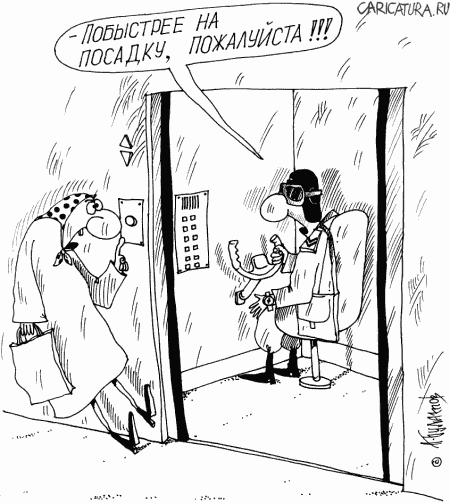
\includegraphics[width=0.9\columnwidth]{./img/posadka}
\end{minipage}
\begin{minipage}[h]{0.7\linewidth}\setlength{\parindent}{1.5em}
    \begin{thm}
    Мальчик Костя живёт в 20-этажном доме. После того, как Костя однажды покатался в лифте, в нём стали работать только две кнопки: «+5» (при нажатии на эту кнопку лифт поднимается на 5 этажей вверх, если это возможно), и «-7» (при нажатии на неё лифт опускается на 7 этажей вниз). Можно ли, пользуясь таким лифтом, попасть
    \par
    а)~с первого этажа на второй? 
    \par
    б)~со второго этажа на первый? 
    \par
    в)~А можно ли вообще пользоваться этим лифтом, т.е. позволяет ли он добираться с любого этажа на любой другой?\footnotemark
    \end{thm}

    \begin{thm} $^{\ast}$ 
    $a, b, c$ - нечётные натуральные числа, не являющиеся квадратами.
    \par
    Может ли число $a^b b^c c^a$ быть полным квадратом?
    \end{thm}
\end{minipage}
\end{figure}
}
\footnotetext{Карикатура из газеты «Большой Новосибирск».}

\begin{thm} $^{\ast\ast}$ 
    Верно ли, что существует число, кратное 2012, и имеющее сумму цифр, равную 2012?
\end{thm}

\begin{thm} $^{\ast}$ 
    Число состоит из 36 цифр. Разрешается разбить его на группы из шести цифр и как-нибудь переставить эти группы. Известно, что одна из перестановок в семь раз больше другой. Докажите, что эта большая перестановка делится на 49.
\end{thm}

\begin{thm} $^{\ast\ast}$ 
    У каждого марсианина три руки и несколько антенн. Несколько марсиан взялись за руки так, что каждый взял за руки трёх других, и все руки при этом оказались заняты. При этом выяснилось, что количество антенн у любых двух взявшихся за руки марсиан отличается ровно в 6 раз. Может ли суммарное количество антенн у марсиан быть ровно 2006?
\end{thm}